\documentclass{beamer}
\usepackage{xeCJK}
\usepackage[xjtu,zh]{collegeBeamer}
\usepackage{booktabs}

\setCJKmainfont[
    Path = C:/Users/10451/AppData/Local/Microsoft/Windows/Fonts/,
    BoldFont = SourceHanSerifSC-Bold.otf,
]{SourceHanSerifSC-Regular.otf}
% when using Chinese, uncomment the following line
% \usepackage{xeCJK}

% meta-data
\title{某医药工厂供电系统设计报告}
\subtitle{电路课大作业报告}
\author{吉致贤\\梅现\\吴政豪}
\date{报告日期:2024.12.26}

% document body
\begin{document}
    
    \maketitle

    \begin{frame}
    本次汇报主要介绍我们小组设计的某医药工厂供电系统,主要包括供电系统的设计思路、设计方案、设计过程、设计结果等内容。

    我们从收集该医药工厂的用电设备信息开始,逐步设计出了适合该公司的供电系统,最终得到了满足该公司用电需求的供电系统设计方案。

    \end{frame}

    \section{背景调查}
    \begin{frame}{工厂工艺概述}{\thesection \, \secname}
        本工程为某医药公司固体制剂项目,项目包括固体制剂大楼、中试车间、
仓库、办公楼以及公用工程项目,固体制剂工艺流程:1:原料准备,包括
药物的接收、检验、粉碎、过筛等步骤。2:制粒,将药物粉末和与辅料混合,通过加水和其它液体粘合剂
制成颗粒。3:干燥:除去制粒过程中的水分和其它容剂,确保颗粒的
稳定性 4:整粒:将干燥颗粒过大过小筛
选,确保颗粒的一致性.5:混合,将不同药物的颗粒均匀混合在一起,以
确保每一种药物都能提供相同的剂量。6:压片或胶囊填充,将混合好的
颗粒通过压片机压成片,或通过胶囊填充机填充。以上六点就是固体制
剂药品大概过程。
\begin{figure}
    \centering
    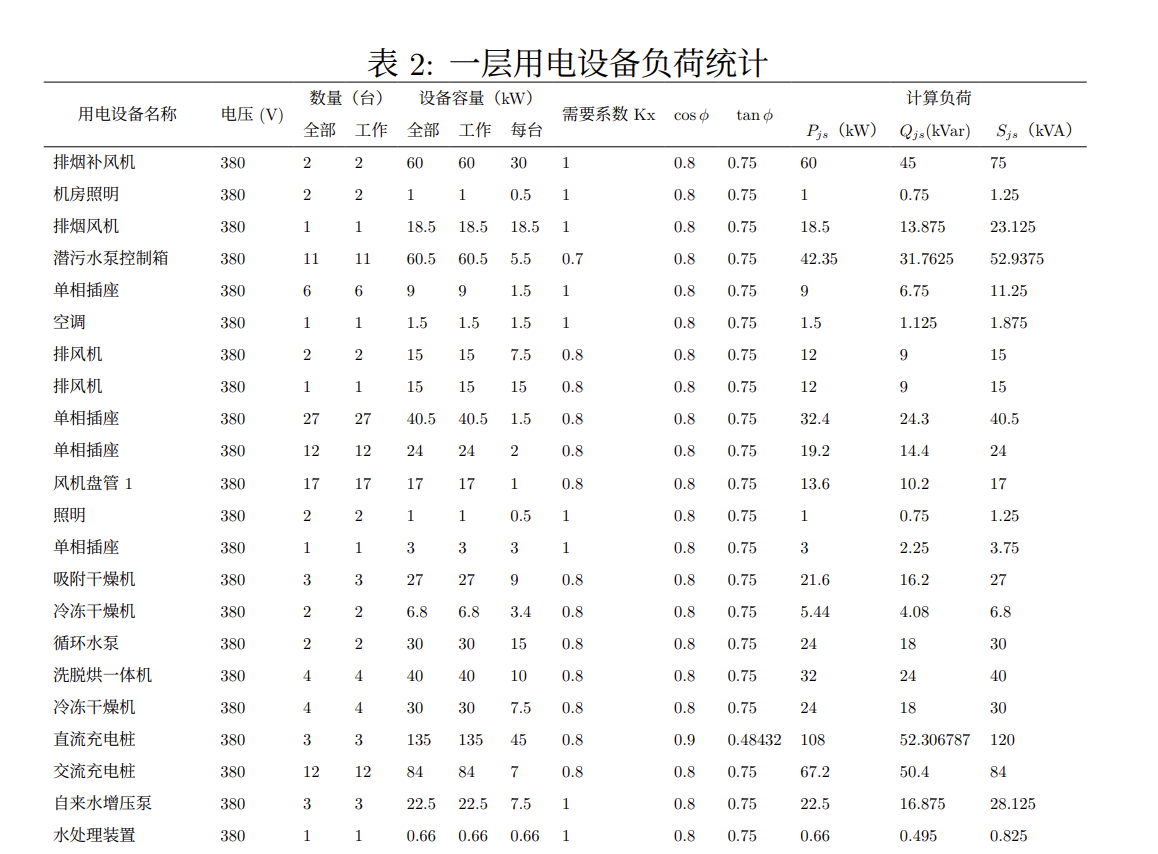
\includegraphics[width=\textwidth]{gallery/1.pdf}
\end{figure}
    \end{frame}

    \begin{frame}{工厂生产概况}{\thesection \, \secname}
    车间年产药片或胶囊 5000 万片或颗,\textbf{二班工作制},\textbf{全年工作 250 天},
每天\textbf{ 8 小时工作制},变压器装机容量 6000kVA, 用电负荷性质为连续工作
制,消防负荷为二级,其它生产用电负荷等级为三级。
    \end{frame}

    \section{供电设计}
    \begin{frame}{供电设计过程}{\thesection \, \secname}
        \begin{enumerate}
            \item 负荷统计,车间所以用电设备负荷统计,包括工艺动力设备、空调动力、照明、电梯等所有用设备。
            \item 根据负荷容量性质,同时使用系数确定全厂用电设备容量,根据用电负荷分布确定变压器容量和电源电压等级。
            \item 确定供电电压等级后绘出高压配电系统图。
            \item 进一步确定电容器电缆等设备的选择,简要根据用电负荷分布在车间合适位置设置终端配置
        \end{enumerate}
        \begin{figure}
            \centering
            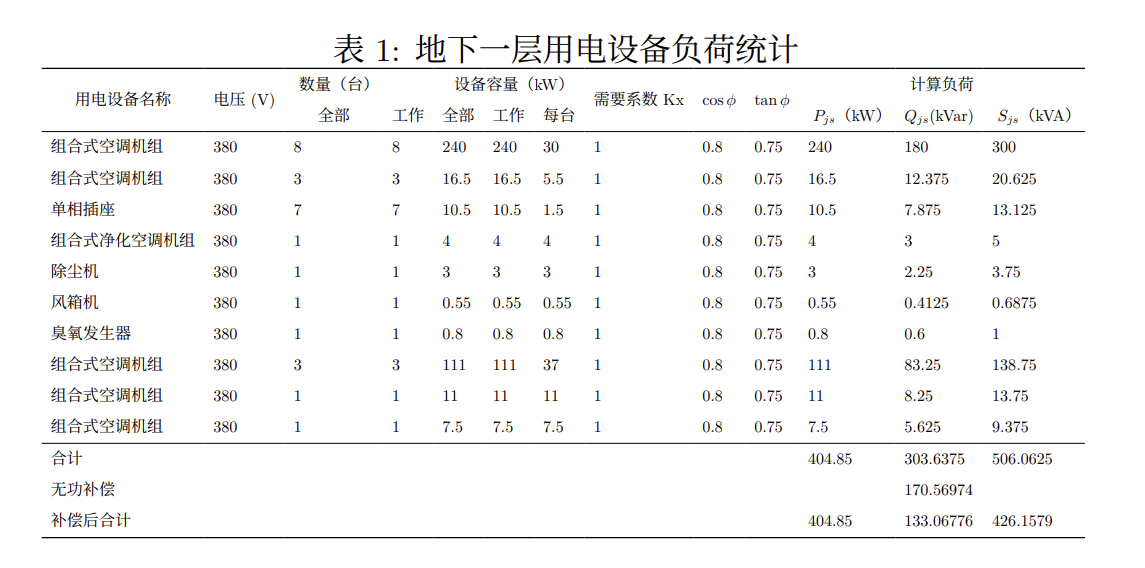
\includegraphics[width=\textwidth]{gallery/2.pdf}
        \end{figure}
    \end{frame}
    \begin{frame}{供电设计}{\thesection \, \secname}
        电源电压为 10kV 两路,设三台干式变压器 2000kVA 变压器一台,1000kVA
变压器二台,一路高压经配电所供到 2000kVA 变压器,配置两个 350kVar
电容器,为整个一楼提供电源;另一路高压经配电所供到两个 1000kVA 变
压器,每一路配置一个 350kVar 的电容器一台变压器为地下一层以及二层
提供电源,另一台变压器为三层以及四层提供电源。
\begin{figure}
            \centering
            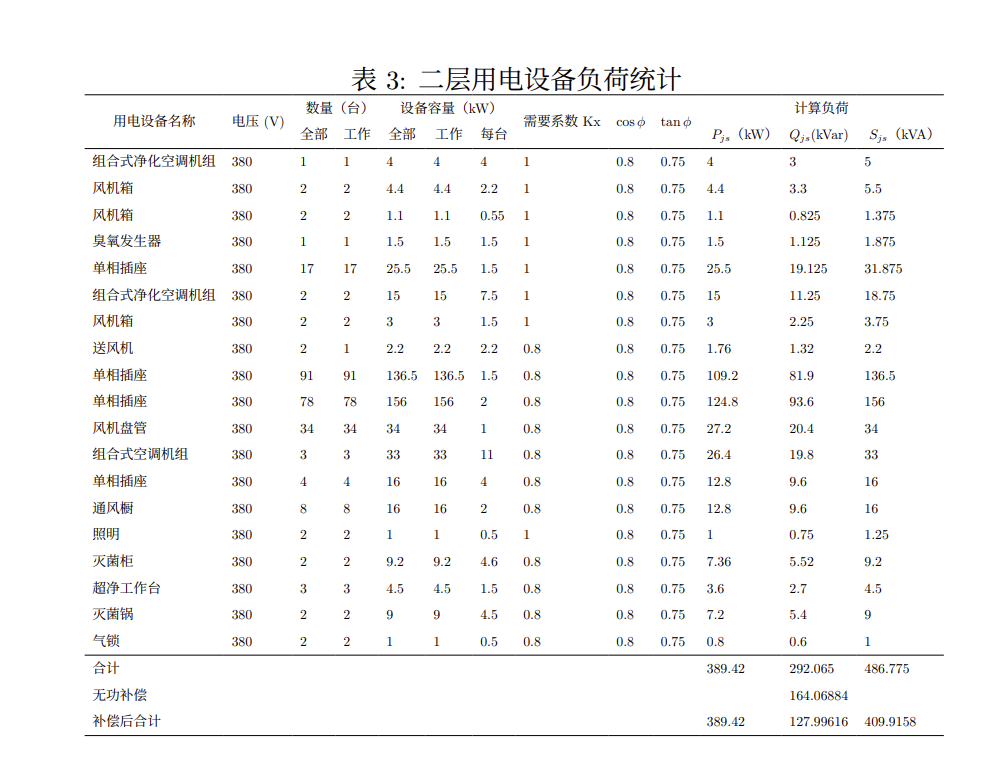
\includegraphics[width=0.6\textwidth]{gallery/3.pdf}
        \end{figure}
    \end{frame}
    \begin{frame}{负荷统计}{\thesection \, \secname}
        \begin{columns}
            \begin{column}{0.4\textwidth}
                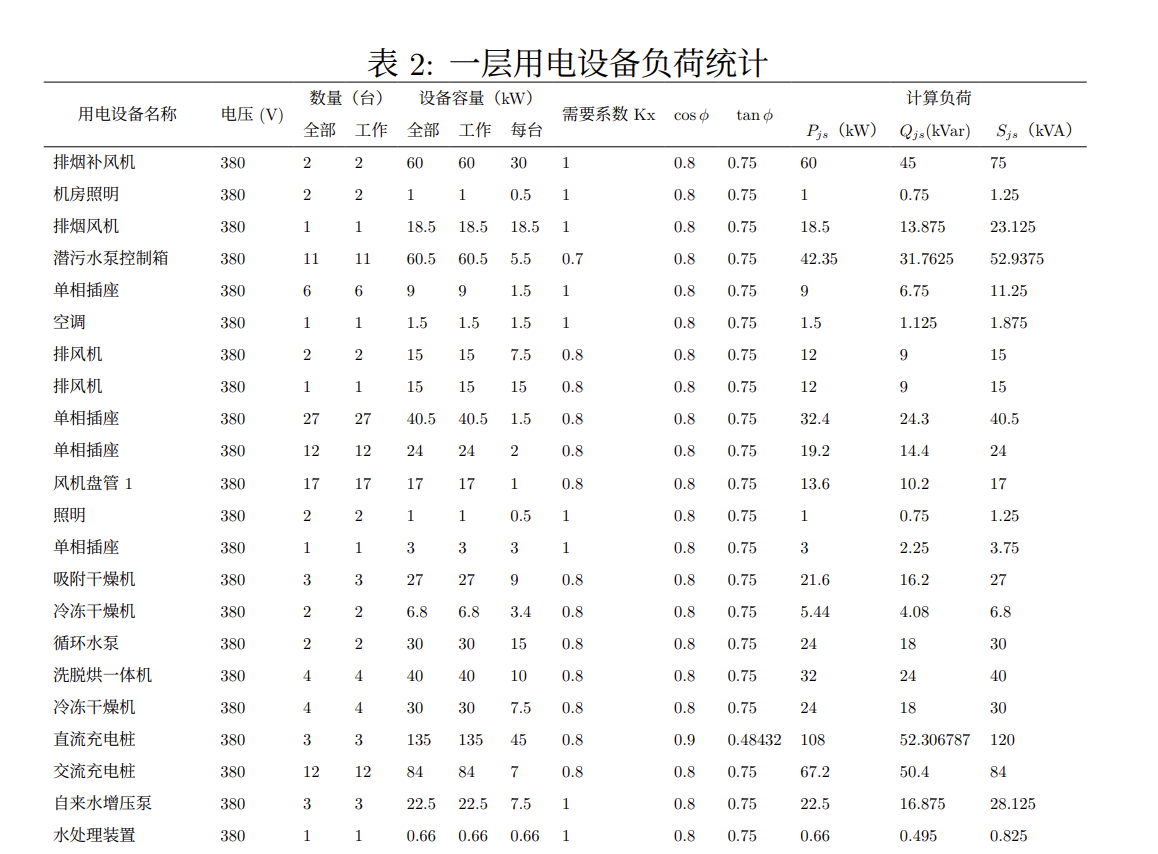
\includegraphics[width=\textwidth]{gallery/1.png}
            \end{column}
            \begin{column}{0.4\textwidth}
                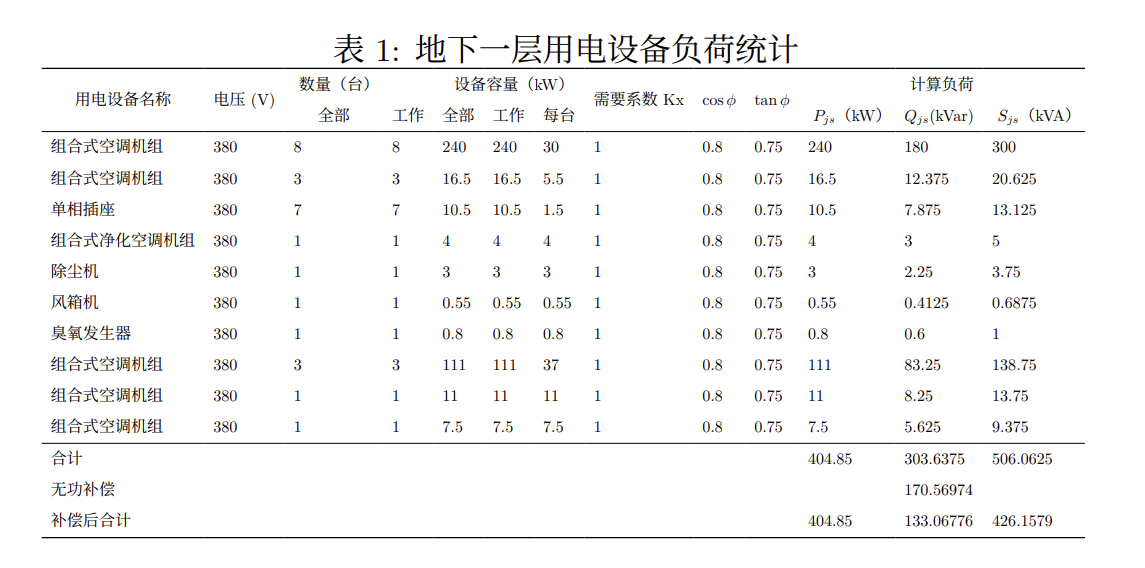
\includegraphics[width=\textwidth]{gallery/2.png}
                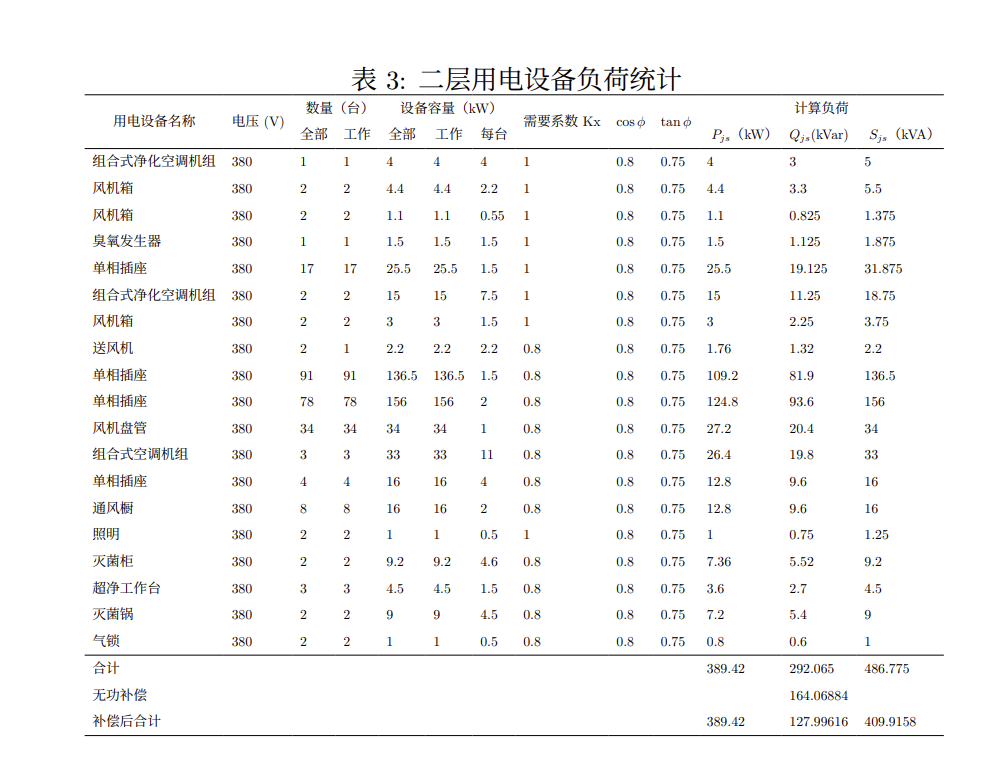
\includegraphics[width=\textwidth]{gallery/3.png}
            \end{column}
        \end{columns}

    \end{frame}
    \begin{frame}{负荷统计}{\thesection \, \secname}
        \begin{columns}
            \begin{column}{0.4\textwidth}
                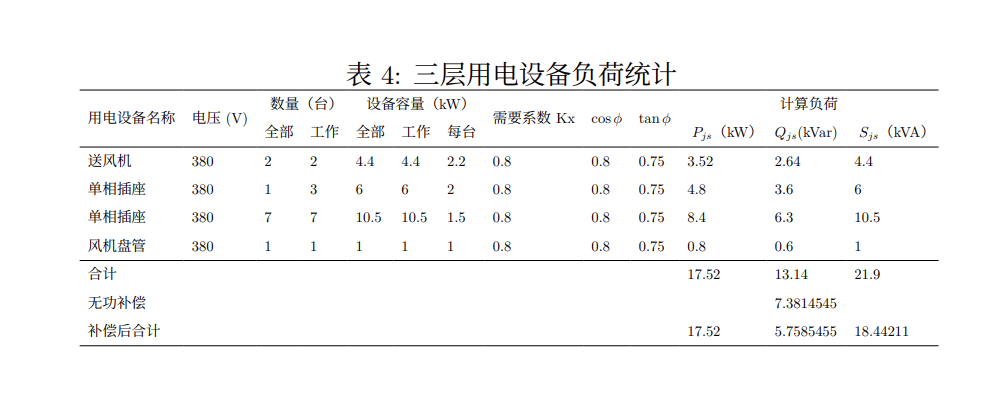
\includegraphics[width=\textwidth]{gallery/4.png}
            \end{column}
            \begin{column}{0.4\textwidth}
                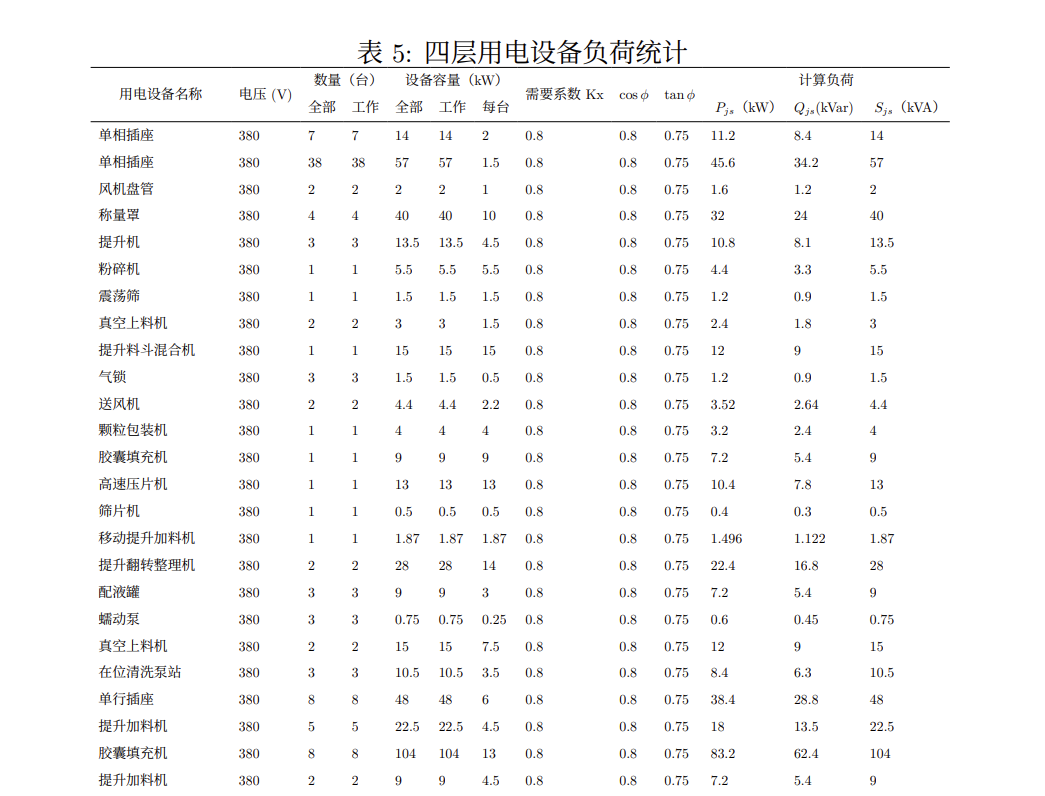
\includegraphics[width=\textwidth]{gallery/5.png}
            \end{column}
        \end{columns}
    \end{frame}

    \section{电路器件的选择}
    \subsection{开关选择}
    \begin{frame}{开关选择}{\thesection \, \secname}
        本医药工厂的设备额定电压均为 380V,并且部分生产设备出厂自带厂
家配置的开关,对于不自带开关的设备,我们给出下列参考开关选择方案:
\begin{enumerate}
    \item 对于\textbf{功率较小}的设备(小于 10kW),可选用 iC60N 3P 25A 或 S203-C25系列开关;
    \item 对于\textbf{中等功率}的设备(10kW 至 50kW),可选用 EZD100F 3P 32A 或Tmax XT1B 3P 32A 系列开关;
    \item 对于\textbf{功率较大}的设备(大于 50kW),可选用 NSX100 3P 50A 或 NM1-100S 3P 50A 系列开关。
\end{enumerate}
    \end{frame}
    \subsection{电容器的选择}
    \begin{frame}{一层的电容器选择}{\thesubsection \, \subsecname}
    经计算得到总有功功率为1610.84kW,总无功功率为1209.65kVar,总视在功率为2014.46kVA,$\cos \phi = 0.80$。

根据相关规定需要将$\cos \phi$提高到0.95,计算得到的补偿无功功率为680.19kVar。

故需要\textbf{两台350kVar的电容器},此时的有功功率为1610.84kW,无功功率为529.46kVar,视在功率为1695.62kVA。
    \end{frame}
    \begin{frame}{地下一层与二层的电容器选择}{\thesubsection \, \subsecname}
    地下一层与二层的总有功功率为794.27kW,总无功功率为595.70kVar,总视在功率为992.84kVA,$\cos \phi = 0.80$。

根据相关规定需要将$\cos \phi$提高到0.95,计算得到的补偿无功功率为334.65kVar。

故可以选用\textbf{一个350kVar的电容器},此时的有功功率为794.27kW,无功功率为245.70kVar,视在功率为831.40kVA。
    \end{frame}
    \begin{frame}{三层与四层的电容器选择}{\thesubsection \, \subsecname}
    经计算得到总有功功率为773.94kW,总无功功率为580.45kVar,总视在功率为967.42kVA,$\cos \phi = 0.80$。

根据相关规定需要将$\cos \phi$提高到0.95,计算得到的补偿无功功率为325.63kVar。

故可以选用\textbf{一个350kVar的电容器},此时的有功功率为773.94kW,无功功率为230.45kVar,视在功率为807.52kVA。

    \end{frame}
    \subsection{变压器与电缆的选择}
    \begin{frame}{一层用电器的变压器与电缆的选择}{\thesubsection \, \subsecname}
    在补偿后得到的视在功率为$S=1695.62\text{kVA}$

考虑到设备线缆磨损导致的潜在负荷增长,取设计常数为1.15:

$$S_{design}= 1.15 \times 1695.62 \approx 1865.18\text{kVA}$$

故可以选择SC10-2000kVA-10/0.4kV变压器。


对于电缆的选择,低压侧电流:

$$I_{low} = \frac{S_{design}}{\sqrt{3} \times U_{low}} = \frac{1865.18}{\sqrt{3} \times 0.4} \approx 2700\text{A}$$

低压侧母线与断路器需要满足2700A的电流,可以选择树脂绝缘母线槽(如 Canalis KR 2700A)
    \end{frame}
\begin{frame}{一层用电器的变压器与电缆的选择}{\thesubsection \, \subsecname}
高压侧电流:

$$I_{high} = \frac{S_{design}}{\sqrt{3} \times U_{high}} = \frac{1865.18}{\sqrt{3} \times 10} \approx 107\text{A}$$

高压侧线缆与断路器需要满足107A的电流,可以选择选择钢带铠装电缆(YJV22 型)型号为3*25$\text{mm}^2$。
    \end{frame}

    \begin{frame}{地下一层与二层用电器的变压器与电缆的选择}{\thesubsection \, \subsecname}
    在补偿后得到的视在功率为$S=831.40\text{kVA}$

考虑到设备线缆磨损导致的潜在负荷增长,取设计常数为1.15:

$$S_{design}= 1.15 \times 831.40 \approx 956.11\text{kVA}$$

故可以选择SC10-1000kVA-10/0.4kV变压器。

对于电缆的选择,低压侧电流:

$$I_{low} = \frac{S_{design}}{\sqrt{3} \times U_{low}} = \frac{956.11}{\sqrt{3} \times 0.4} \approx 1380\text{A}$$

低压侧母线与断路器需要满足1380A的电流,可以选择树脂绝缘母线槽(如 Canalis KR 1600A)
    \end{frame}
\begin{frame}{地下一层与二层用电器的变压器与电缆的选择}{\thesubsection \, \subsecname}
高压侧电流:

$$I_{high} = \frac{S_{design}}{\sqrt{3} \times U_{high}} = \frac{956.11}{\sqrt{3} \times 10} \approx 55\text{A}$$

高压侧线缆与断路器需要满足55A的电流,可以选择YJV-8.7/15kV 3×50$\text{mm}^2$。
    \end{frame}



\begin{frame}{三层与四层用电器的变压器与电缆的选择}{\thesubsection \, \subsecname}
    在补偿后得到的视在功率为$S=807.52\text{kVA}$

考虑到设备线缆磨损导致的潜在负荷增长,取设计常数为1.15:

$$S_{design}= 1.15 \times 807.52 \approx 928.15\text{kVA}$$

故可以选择SC10-1000kVA-10/0.4kV变压器。

对于电缆的选择,低压侧电流:

$$I_{low} = \frac{S_{design}}{\sqrt{3} \times U_{low}} = \frac{928.15}{\sqrt{3} \times 0.4} \approx 1340\text{A}$$

低压侧母线与断路器需要满足1340A的电流,可以选择树脂绝缘母线槽(如 Canalis KR 1600A)
    \end{frame}
\begin{frame}{三层与四层用电器的变压器与电缆的选择}{\thesubsection \, \subsecname}
高压侧电流:

$$I_{high} = \frac{S_{design}}{\sqrt{3} \times U_{high}} = \frac{928.15}{\sqrt{3} \times 10} \approx 53\text{A}$$

高压侧线缆与断路器需要满足53A的电流,可以选择YJV-8.7/15kV 3×50$\text{mm}^2$。
    \end{frame}

\section{总结与感想}
\begin{frame}{总结与感想}{\thesection \, \secname}
    本次设计中,我们小组首先对医药工厂的用电设备进行了详细的调查,然后根据工厂的用电需求,设计出了适合该工厂的供电系统。

    在设计过程中,我们小组充分利用了所学的电路知识,对供电系统的设计进行了详细的分析,最终得到了满足工厂用电需求的供电系统设计方案。

    通过本次设计,我们小组不仅加深了对电路知识的理解,还提高了我们的动手能力和团队合作能力,为我们今后的学习和工作打下了坚实的基础。
\end{frame}
\end{document}